% Soubory musí být v kódování, které je nastaveno v příkazu \usepackage[...]{inputenc}

\documentclass[%
%  draft,    				  % Testovací překlad
  12pt,       				% Velikost základního písma je 12 bodů
  a4paper,    				% Formát papíru je A4
%  oneside,      			% Jednostranný tisk (výchozí)
%% Z následujicich voleb lze použít maximálně jednu:
%	dvipdfm  						% výstup bude zpracován programem 'dvipdfm' do PDF
%	dvips	  						% výstup bude zpracován programem 'dvips' do PS
%	pdftex							% překlad bude proveden programem 'pdftex' do PDF (výchozí)
	unicode,						% Záložky a informace budou v kódování unicode
%% Z následujících voleb lze použít jen jednu:
%english,            % originální jazyk je angličtina
czech              % originální jazyk je čeština (výchozí)
%slovak,             % originální jazyk je slovenčina
]{report}				    	% Dokument třídy 'zpráva'

\usepackage[utf8]		%	Kódování zdrojových souborů je v UTF-8
	{inputenc}					% Balíček pro nastavení kódování zdrojových souborů

\usepackage{graphicx} % Balíček 'graphicx' pro vkládání obrázků
											% Nutné pro vložení log školy a fakulty

\usepackage[
	nohyperlinks				% Nebudou tvořeny hypertextové odkazy do seznamu zkratek
]{acronym}						% Balíček 'acronym' pro sazby zkratek a symbolů
											% Nutné pro použití prostředí 'seznamzkratek' balíčku 'thesis'

\usepackage[
	breaklinks=true,		% Hypertextové odkazy mohou obsahovat zalomení řádku
	hypertexnames=false % Názvy hypertextových odkazů budou tvořeny
											% nezávisle na názvech TeXu
]{hyperref}						% Balíček 'hyperref' pro sazbu hypertextových odkazů
											% Nutné pro použití příkazu 'nastavenipdf' balíčku 'thesis'

\usepackage{pdfpages} % Balíček umožňující vkládat stránky z PDF souborů
                      % Nutné při vkládání titulních listů a zadání přímo
                      % ve formátu PDF z informačního systému

\usepackage{enumitem} % Balíček pro nastavení mezerování v odrážkách
  \setlist{topsep=0pt,partopsep=0pt,noitemsep}

\usepackage{cmap} 		% Balíček cmap zajišťuje, že PDF vytvořené `pdflatexem' je
											% plně "prohledávatelné" a "kopírovatelné"

\usepackage{upgreek}	% Balíček pro sazbu stojatých řeckých písmem
											% např. stojaté pí: \uppi
											% např. stojaté mí: \upmu (použitelné třeba v mikrometrech)
											% pozor, grafická nekompatibilita s fonty typu Computer Modern!

\usepackage{dirtree}		% sazba adresářové struktury

\usepackage[formats]{listings}	% Balíček pro sazbu zdrojových textů
\lstset{
%	Definice jazyka použitého ve výpisech
%    language=[LaTeX]{TeX},	% LaTeX
%	language={Matlab},		% Matlab
	language={C},           % jazyk C
    basicstyle=\ttfamily,	% definice základního stylu písma
    tabsize=2,			% definice velikosti tabulátoru
    inputencoding=utf8,         % pro soubory uložené v kódování UTF-8
    %inputencoding=cp1250,      % pro soubory uložené ve standardním kódování Windows CP1250
		columns=fixed,  %flexible,
		fontadjust=true %licovani sloupcu
    extendedchars=true,
    literate=%  definice symbolů s diakritikou
    {á}{{\'a}}1
    {č}{{\v{c}}}1
    {ď}{{\v{d}}}1
    {é}{{\'e}}1
    {ě}{{\v{e}}}1
    {í}{{\'i}}1
    {ň}{{\v{n}}}1
    {ó}{{\'o}}1
    {ř}{{\v{r}}}1
    {š}{{\v{s}}}1
    {ť}{{\v{t}}}1
    {ú}{{\'u}}1
    {ů}{{\r{u}}}1
    {ý}{{\'y}}1
    {ž}{{\v{z}}}1
    {Á}{{\'A}}1
    {Č}{{\v{C}}}1
    {Ď}{{\v{D}}}1
    {É}{{\'E}}1
    {Ě}{{\v{E}}}1
    {Í}{{\'I}}1
    {Ň}{{\v{N}}}1
    {Ó}{{\'O}}1
    {Ř}{{\v{R}}}1
    {Š}{{\v{S}}}1
    {Ť}{{\v{T}}}1
    {Ú}{{\'U}}1
    {Ů}{{\r{U}}}1
    {Ý}{{\'Y}}1
    {Ž}{{\v{Z}}}1
}

%% Nastavení českého jazyka při sazbě v češtině.
% Pro sazbu češtiny je možné použít mezinárodní balíček 'babel', jenž
% použití doporučujeme pro nové instalace (MikTeX2.8,TeXLive2009), nebo
% národní balíček 'czech', který doporučujeme ve starších instalacích.
% Balíček 'babel' bude správně fungovat pouze ve spojení s programy
% 'latex', 'pdflatex', zatímco balíček 'czech' bude fungovat ve spojení
% s programy 'cslatex', 'pdfcslatex'.
% Varianta A:
\usepackage    				
  {babel}             % Balíček pro sazbu různojazyčných dokumentů; kompilovat (pdf)latexem!
  										% převezme si z parametrů třídy správný jazyk
\usepackage{lmodern}	% vektorové fonty Latin Modern, nástupce půvoních Knuthových Computern Modern fontů
\usepackage{textcomp} % Dodatečné symboly
\usepackage[T1]{fontenc}  % Kódování fontu - mj. kvůli správným vzorům pro dělení slov
% Varianta B:
%\usepackage{czech}   % Alternativní balíček pro sazbu v českém jazyce, kompilovat (pdf)cslatexem!
\usepackage{xcolor}

\usepackage[%
%% Z následujících voleb lze použít pouze jednu
% left,               % Rovnice a popisky plovoucich objektů budou %zarovnány vlevo
  center,             % Rovnice a popisky plovoucich objektů budou zarovnány na střed (vychozi)
%% Z následujících voleb lze použít pouze jednu
semestral						%	sazba zprávy semestrálního projektu
%bachelor						%	sazba bakalářské práce
%diploma						 % sazba diplomové práce
%treatise            % sazba pojednání o dizertační práci
%phd                 % sazba dizertační práce
]{thesis}             % Balíček pro sazbu studentských prací
                      % Musí být vložen až jako poslední, aby
                      % ostatní balíčky nepřepisovaly jeho příkazy

%%%%%%%%%%%%%%%%%%%%%%%%%%%%%%%%%%%%%%%%%%%%%%%%%%%%%%%%%%%%%%%%%
%%%%%%      Definice informací o dokumentu             %%%%%%%%%%
%%%%%%%%%%%%%%%%%%%%%%%%%%%%%%%%%%%%%%%%%%%%%%%%%%%%%%%%%%%%%%%%%

%% Název práce:
%  První parametr je název v originálním jazyce,
%  druhý je překlad v angličtině nebo češtině (pokud je originální jazyk angličtina)
\nazev{Generátor kybernetických útoků}{Cyberattack generator}

%% Jméno a příjmení autora ve tvaru
%  [tituly před jménem]{Křestní}{Příjmení}[tituly za jménem]
\autor{Ondřej}{Gajdušek}

%% Jméno a příjmení vedoucího/školitele včetně titulů
%  [tituly před jménem]{Křestní}{Příjmení}[tituly za jménem]
% Pokud osoba nemá titul za jménem, smažte celý řetězec '[...]'
\vedouci[doc.\ Ing.]{Jan}{Hajný}[Ph.D.]

%% Jméno a příjmení oponenta včetně titulů
%  [tituly před jménem]{Křestní}{Příjmení}[tituly za jménem]
% Pokud nemá titul za jménem, smažte celý řetězec '[...]'
% Uplatní se pouze v prezentaci k obhajobě;
% v případě, že nechcete, aby se na titulním snímku prezentace zobrazoval oponent, pouze jej zakomentujte;
% u obhajoby semestrální práce se oponent nezobrazuje
\oponent[doc.\ Mgr.]{Křestní}{Příjmení}[Ph.D.]

%% Označení oboru studia
% První parametr je obor v originálním jazyce,
% druhý parametr je překlad v angličtině nebo češtině
\oborstudia{Informační bezpečnost}{Information security}

%% Označení fakulty
% První parametr je název fakulty v originálním jazyce,
% druhý parametr je překlad v angličtině nebo v češtině
%\fakulta{Fakulta architektury}{Faculty of Architecture}
\fakulta{Fakulta elektrotechniky a komunikačních technologií}{Faculty of Electrical Engineering and Communication}
%\fakulta{Fakulta chemická}{Faculty of Chemistry}
%\fakulta{Fakulta informačních technologií}{Faculty of Information Technology}
%\fakulta{Fakulta podnikatelská}{Faculty of Business and Management}
%\fakulta{Fakulta stavební}{Faculty of Civil Engineering}
%\fakulta{Fakulta strojního inženýrství}{Faculty of Mechanical Engineering}
%\fakulta{Fakulta výtvarných umění}{Faculty of Fine Arts}

%% Označení ústavu
% První parametr je název ústavu v originálním jazyce,
% druhý parametr je překlad v angličtině nebo češtině
%\ustav{Ústav automatizace a měřicí techniky}{Department of Control and Instrumentation}
%\ustav{Ústav biomedicínského inženýrství}{Department of Biomedical Engineering}
%\ustav{Ústav elektroenergetiky}{Department of Electrical Power Engineering}
%\ustav{Ústav elektrotechnologie}{Department of Electrical and Electronic Technology}
%\ustav{Ústav fyziky}{Department of Physics}
%\ustav{Ústav jazyků}{Department of Foreign Languages}
%\ustav{Ústav matematiky}{Department of Mathematics}
%\ustav{Ústav mikroelektroniky}{Department of Microelectronics}
%\ustav{Ústav radioelektroniky}{Department of Radio Electronics}
%\ustav{Ústav teoretické a experimentální elektrotechniky}{Department of Theoretical and Experimental Electrical Engineering}
\ustav{Ústav telekomunikací}{Department of Telecommunications}
%\ustav{Ústav výkonové elektrotechniky a elektroniky}{Department of Power Electrical and Electronic Engineering}

\logofakulta[loga/FEKT_zkratka_barevne_PANTONE_CZ]{loga/UTKO_color_PANTONE_CZ}


%% Rok obhajoby
\rok{2017}
\datum{1.\,1.\,1970} % Datum se uplatní pouze v prezentaci k obhajobě

%% Místo obhajoby
% Na titulních stránkách bude automaticky vysázeno VELKÝMI písmeny
\misto{Brno}

%% Abstrakt
\abstrakt{Abstrakt práce v~originálním jazyce
}{Překlad abstraktu v~angličtině (nebo češtině pokud je originální jazyk angličtina)
}

%% Klíčová slova
\klicovaslova{Klíčová slova v~originálním jazyce}%
	{Překlad klíčových slov v~angličtině nebo češtině}

%% Poděkování
\podekovanitext{Rád bych poděkoval vedoucímu diplomové práce panu doc. Ing.~Janu Hajnému, Ph.D.\ za odborné vedení, konzultace, trpělivost a podnětné návrhy k~práci.}  % do tohoto souboru doplňte údaje o sobě, o názvu práce...

%%%%%%%%%%%%%%%%%%%%%%%%%%%%%%%%%%%%%%%%%%%%%%%%%%%%%%%%%%%%%%%%%%%%%%%%

%%%%%%%%%%%%%%%%%%%%%%%%%%%%%%%%%%%%%%%%%%%%%%%%%%%%%%%%%%%%%%%%%%%%%%%%
%%%%%%     Nastavení polí ve Vlastnostech dokumentu PDF      %%%%%%%%%%%
%%%%%%%%%%%%%%%%%%%%%%%%%%%%%%%%%%%%%%%%%%%%%%%%%%%%%%%%%%%%%%%%%%%%%%%%
%% Při vloženém balíčku 'hyperref' lze použít příkaz '\nastavenipdf'
\nastavenipdf
%  Nastavení polí je možné provést také ručně příkazem:
%\hypersetup{
%  pdftitle={Název studentské práce},    	% Pole 'Document Title'
%  pdfauthor={Autor studenstké práce},   	% Pole 'Author'
%  pdfsubject={Typ práce}, 						  	% Pole 'Subject'
%  pdfkeywords={Klíčová slova}           	% Pole 'Keywords'
%}
%%%%%%%%%%%%%%%%%%%%%%%%%%%%%%%%%%%%%%%%%%%%%%%%%%%%%%%%%%%%%%%%%%%%%%%

%%%%%%%%%%%%%%%%%%%%%%%%%%%%%%%%%%%%%%%%%%%%%%%%%%%%%%%%%%%%%%%%%%%%%%%
%%%%%%%%%%%       Začátek dokumentu               %%%%%%%%%%%%%%%%%%%%%
%%%%%%%%%%%%%%%%%%%%%%%%%%%%%%%%%%%%%%%%%%%%%%%%%%%%%%%%%%%%%%%%%%%%%%%
\begin{document}


%% Vložení desek generovaných informačním systémem
%\includepdf[pages=1,offset=15.4mm -1in]%
%  {pdf/student-desky}% název souboru nesmí obsahovat mezery!
% nebo vytvoření desek z balíčku
%\vytvorobalku
\setcounter{page}{1} %resetovani citace stranek - desky se necisluji

%% Vložení titulního listu generovaného informačním systémem
\includepdf[pages=1,offset=15.4mm -1in]%
  {pdf/student-titulka}% název souboru nesmí obsahovat mezery!
% nebo vytvoření titulní stránky z balíčku
%\vytvortitulku
   
%% Vložení zadání generovaného informačním systémem
%\includepdf[pages=1,offset=15.4mm -1in]%
%  {pdf/student-zadani}% název souboru nesmí obsahovat mezery!
% nebo lze vytvořit prázdný list příkazem ze šablony
%\stranka{}%
%	{\sffamily\Huge\centering ZDE VLOŽIT LIST ZADÁNÍ}%
%	{\sffamily\centering Z~důvodu správného číslování stránek}

%% Vysázení stránky s abstraktem
\vytvorabstrakt

%% Vysázení prohlaseni o samostatnosti
\vytvorprohlaseni

%% Vysázení poděkování
\vytvorpodekovani

%% Vysázení poděkování projektu SIX
% ----------- zakomentujte pokud neodpovida realite
\vytvorpodekovaniSIX

% Poděkování KA6

\includepdf[pages=1,offset=15.4mm -1in]{pdf/podekovani_OPVVV_BP_DP.pdf}

%% Vysázení obsahu
\obsah

%% Vysázení seznamu obrázků
\seznamobrazku

%% Vysázení seznamu tabulek
\seznamtabulek

%% Vysázení seznamu výpisů
\lstlistoflistings

%% Vložení souboru 'text/uvod.tex' s úvodem
% !TeX spellcheck = cs_CZ
\chapter*{Úvod}
\phantomsection
\addcontentsline{toc}{chapter}{Úvod}


V~dnešní době, kdy existují jisté iniciativy, které chtějí prosadit internet jako právo, je internet 
pro moderního člověka, jeho denní činnosti, i firmy prakticky neodmyslitelný \cite{pirati_internet}. 
Dotčeny jsou nejen oblasti podnikání ale také oblasti vzdělání, umění a další. Výpadek této služby má 
mnohdy nepředstavitelné následky jako finanční ztrátu nebo mnohem citelnější jako nefunkčnost eshopů, 
bankovních či jiných informačních systémů. Za těmito výpadky můžeme nejčastěji hledat kybernetický útok, 
což je promyšlené škodlivé jednání útočníků zaměřené na  IT  infrastrukturu  za  účelem  způsobit 
poškození  a  získat  citlivé  či  strategicky  důležité 
informace promyšlené nebo naplnit určitý sociální, ideologický, náboženský, politický nebo jiný záměr 
\cite{Jirasek2012}. Čím více je fungování společnosti na internetu závislejší, tím více jsou tyto hrozby 
závažnější a je třeba se jimi zabývat. Nejčastějším typem útoku je \zkratka{zk_dos}, proti kterému 
v~mnoha případech neexistuje  žádná spolehlivá obrana \cite{akamai_q2_2017}. Útoky tohoto typu mají 
za cíl znepřístupnit danou službu běžící na serveru nebo server samotný, pro běžného uživatele se tak 
tváří býti nedostupný. Útočníkem se může stát kdokoli, ať už je to běžný uživatel, síťový expert nebo 
v~také organizovaná skupina útočníků. Právě tyto skupiny jsou schopny docílit většího efektu a jsou 
schopny napáchat větší škody. Cíl útoku nemusí nutně být národního či nadnárodního rozměru.

Je zjevné, že kybernetickou bezpečnost nelze podcenit a bezesporu zaujímá neméně důležitou roli. Tato 
práce se zabývá popisem \zkratkatext{zk_dos} útoků a rozšířením softwarového generátoru kybernetických útoků 
o~nové typy útoků.

První část popisuje \zk{zk_dos} útoky, přiblížím jejich původ, fungování. Implementované typy útoků 
popíši detailněji.

% !TeX spellcheck = cs_CZ
\chapter[DoS útoky]{DoS útoky}
V~této kapitole budou rozebrány \zk{zk_dos} útoky, jejich princip, charakteristika a následně
dělení. Dále tato kapitola zmiňuje využití \zk{zk_ddos} útoků jako služby. V~závěru jsou
zmíněny implementované útoky.

\section{Charakteristika}
\zk{zk_dos} lze charakterizovat jako kybernetický útok, který si klade za cíl znepřístupnění
 cílové služby legitimním uživatelům. Využívají jedné nebo více zranitelností v~implementaci
 konkrétního software. Ve své podstatě každá stanice se může stát cílem, obětí, útoku
 \zk{zk_dos}. \zk{zk_dos} útoky se mezi útočníky velmi rychle staly populárními a tento trend
 se nemění \cite{akamai_q2_2017}. Realizace \zk{zk_dos} útoku není nikterak obtížná a
 nevyžaduje z~útočníkovy strany hluboké znalosti, jelikož nástroje k~jejich provedení jsou
 běžně dostupné, viz. kapitola \ref{chap:nastroje_pro_dos}. Fakt, že narušit činnost sítě bývá
 jednodušší, než do ní získat přístup podporuje tento trend a jejich rozšířenost. 

Motivy takových útoků mohou být hacktivizmus, vydírání, nekalé konkurenční praktiky,
zlomyslnost nebo smokescreen coby prostředek krytí jiného současně prováděného útoku nebo
určitá forma protestu. Dalšími motivy mohou být také uznání hackerské komunity nebo také
politické politický motiv.

Velká část útoků využívá nedostatků v~architektuře rodiny protokolů TCP/IP, které byly k~tomu,
aby byly funkční, nikoliv bezpečné. Používaly se v~otevřeném a důvěryhodném prostředí, čemuž
v~dnešní době není.

Trend naznačuje rostoucí počet druhu a implementací jednotlivých útoků, proto bychom měli
věnovat pozornost a určité úsilí na ochranu proti nim. Útočník je ve výhodě, jelikož nelze
jednoznačně predikovat cíl jeho útoku.


\section{Typy útoků}
\subsection{Útok z~jednoho zdroje a útok distribuovaný}
\zk{zk_dos} útoky mohou být prováděny z~jednoho místa, což je méně časté, jelikož při
\zk{zk_dos} útoku není útočník z~důvodu malé šířky pásma schopen vygenerovat dostatečný síťový
provoz na to, aby způsobil odepření služby na cíli svého útoku. Lze tedy jeho účinek znásobit a
to použitím většího počtu útočících stanic. Takový útok nazýváme \zkratka{zk_ddos}. V~případě
\zk{zk_dos} útoku není útočník mnohdy schopen vygenerovat dostatečný síťový provoz na to, aby
způsobil odepření služby na cíli svého útoku.

Pro distribuovaný \zk{zk_dos} útok je charakteristický velmi vysoký počet uživatelských stanic,
či serverů, použitých k~realizaci tohoto útoku. Pohybujeme se v~řádech desítek, stovek až
milionů počítačů. 
Často jsou tyto počítače napadeny virem, trojským koněm nebo programem, který v~sobě ukrývá
skrytou funkci a následně jsou zneužitý k~účelům \zk{zk_dos} útoku bez vědomí jejich majitele.
Zajímavým cílem útočníků jsou zařízení IoT, které útočník může následně využít k~\zk{zk_dos}
útoku.

Takové stanice nazýváme \uv{boti} a seskupení více těchto stanic \uv{botnety}. Důvody pro
vytvoření botnetu jsou větší šířka pásma, šíření spamu nebo redistribuce malware nejen do sítě,
kde se \uv{bot} nachází. Tito \uv{boti} jsou zapojeni do \zkratka{zk_cnc} infrastruktury spolu
s~\zkratka{zk_irc} servery skrze které může útočník rozesílat instrukce botům. %TODO:zdroj
\zk{zk_irc} servery poskytují centralizovanou správu botů nebo celých botnetů skrze \zk{zk_cnc}
mechanizmy. Jedním z mnoha trojských koní je Linux.Kaiten. Jedná se o klienta ovládaného skrze
\zk{zk_irc} server, který může stahovat a spouštět soubory, provádět \zk{zk_ddos} útoky za
použití UDP Flood a SYN Flood útoků a také umožňuje spoofing IP adresy.

Útoky vedené skrze tyto botnety dokáží plně zahltit šířku pásma oběti a způsobí tak odepření
služby. 
Boti mohou být rozmístěni kdekoli po světě, což znesnadňuje ochranu tím, že nelze
jednoznačně podle geolokační stopy IP adresy filtrovat provoz z~konkrétní země, což je
podpořeno možností měnit zdrojovou adresu v~IP datagramu, tzv. IP spoofing.
%TODO:obrazek utoku za pomoci spoofovane ip adresy
%TODO:zde vlozit obrazek ddos utoku

\subsection{Zesílené útoky}
\subsubsection{Reflektované útoky}
\label{subsec:reflektovane_utoky}
K~zesílení útoku lze použít \uv{reflektor}. Reflektor je prvek v~síti, který reflektuje provoz
iniciovaný ze strany útočníka. Při takovém útoku je \uv{spoofována} zaměněna zdrojovoá adresa
v~IP datagramu. Útočník při trojcestném handshakingu (three-way handshake) zasílá na reflektor
paket s~příznakem SYN se spoofovanou adresou, ten následně odpoví paketem s~příznakem SYN/ACK
na podvrženou IP adresu, tedy adresou oběti. Reflektor tak neodesílá odpověď útočníkovi ale
oběti. Při dostatečném počtu odeslaných žádostí směrem k~oběti dochází k~vyčerpání zdrojů, tedy
k~odepření služby. Oběť se tak může domnívat, že na ni útočí reflektory. Pravý útočník zůstává
skryt. Reflektovaný útok lze označit jako \zkratka{zk_drdos}.

\subsubsection{Amplifikované útoky}
Jiným typem jsou takzvané \uv{amplifikované} útoky, které využívají \uv{amplifikátoru}.
\uv{Amplifikátor} amplifikuje, tedy zvětšuje síťový provoz zaslaný útočníkem a zasílá jej na
spoofovanou IP adresu oběti, což tento útok činí silnějším než je přímý útok. Útočník je díky
tomuto schopen vygenerovat dostatečný síťový provoz pro zahlcení oběti.

Příkladem takové amplifikace může být například dotaz na DNS server, v~jehož zóně se nachází
rozsáhlý TXT záznam. Nebo v~případě \zkratka{zk_ntp} serveru si můžeme zažádat o~posledních~600
adres, které se k~němu připojily. Následující tabulka \ref{tab:udp_ampl} zobrazuje,
kolikanásobně je větší odpověď od reflektoru oproti vyslané žádosti směrem k~němu.

\begin{table}[]
	\centering
	\caption{Amplifikační útoky založené na UDP \cite{TA14-017A}}
	\label{tab:udp_ampl}
	\begin{tabular}{|l|l|}
		\hline
		Protokol               & Faktor zvětšení šířky pásma    \\ \hline
		NTP                    & 556.9                          \\ \hline
		CharGen                & 358.8                          \\ \hline
		DNS                    & do 179                         \\ \hline
		QOTD                   & 140.3                          \\ \hline
		Quake Network Protocol & 63.9                           \\ \hline
		BitTorrent             & 4.0 - 54.3                     \\ \hline
		SSDP                   & 30.8                           \\ \hline
		Kad                    & 16.3                           \\ \hline
		SNMPv2                 & 6.3                            \\ \hline
		Steam Protocol         & 5.5                            \\ \hline
		NetBIOS                & 3.8                            \\ \hline
	\end{tabular}
\end{table}

Pro větší účinek těchto zesílených útoků lze využít namísto \zk{zk_dos} útoku útok \zk{zk_ddos}.

\section{Dělení útoků}
%Útoky lze také specifikovat a rozdělit podle TCP/IP vrstev, skrze které působí.
\subsection{Podle počtu útočících zařízení}

\subsection{Podle spotřeby zdrojů}

\subsection{Podle rychlosti}

\subsection{Podle spoje}
%spojované a nespojované

\section{DDoS jako služba}
Dnes uživateli běžně přístupné služby v podobě \zk{zk_dos} nebo \zk{zk_ddos} útoků poskytované
konkrétními službami lze nazvat \zkratka{zk_ddosaas}.

Definuji sebe sama jako službu stresového testování přičemž po objednateli této služby není
vyžadována znalost datových sítí. Ve smluvních podmínkách se zříkají odpovědnosti za škody
způsobené objednateli. Přičemž ani nezjišťují, zda cíl útoku, který si zákazník objednal je či
není v jeho správě. Vyžadují registraci a za úplatu poskytují stresové testování. Platbu je
možno provádět buď v Bitcoinech nebo přes PayPal. Ceny za tuto službu se pohybují přibližně v
rozmezí mezi 2-10 americkými dolary. Mnoho takových služeb nabízí i podporu typu 24/7 skrze
\zkratka{zk_im}. Dostupných bývá povětšinou pár základních útoků založených na protokolech
\zkratka{zk_tcp}, \zkratka{zk_udp} a \zkratka{zk_http}. Tyto služby využívají také IP spoofing
a zesílení útoku pomocí amplifikátorů \ref{subsec:reflektovane_utoky}. 

Největší hrozbou \zk{zk_ddosaas} útoků je jejich snadná dostupnost. Avšak tyto útoky nejsou
nikterak sofistikované a nejsou příliš velkou hrozbou pro standardně zabezpečenou síť
\cite{DDoSaaS}.

\section{Útoky mířené na síťové zdroje}

\subsection{Záplavové}

\section{Útoky mířené na serverové zdroje}
% jak funguje normalne, slabina v tcp/ip, pomale utoky

\section{Útoky mířené na aplikační zdroje}
Tyto typy útoků se zaměřují na zranitelnosti aplikace samotné aplikace vystupující na 7. vrstvě ISO/OSI modelu. Využívají zranitelností v implementaci samotného aplikačního protokolu nebo aplikace běžící na cílovém serveru. Tato zranitelnost nemusí nutně býti implementační chybou ale jen slabým místem, kterého lze využít. Kupříkladu vyšlu na serverpožadavek, jež je na straně serveru nutno zpracovat a do této akce velké množství výpočetních zdrojů. Je-li takovýchto příchozích žádostí na server vysláno více, dochází na jeho straně k vyčerpání výočetních zdrojů, nelze zpracovat požadavky legitimních uživatelů, čímž dochází k odepření služby a tedy k úspěšnému DoS útoku.


Příkladem takových útoků může být HTTP GET, který

Dalším útokem cílícím na aplikační zdroje je

Do této kategorie útoků lze zařadit taky útok XX
%HTTP GET!!
%http
%%vice druhu http utoku
%slow loris?
%slow read?

\section{Implementované útoky}
V této kapitole jsou rozebrány útoky, které byly implementovány do aplikace DoSGen.

\subsection{NTP flood}
Tento útok využívá funcke monlist, která vrací seznam IP adres posledních 600 klientů připojených k NTP serveru.




%\chapter{Nástroje pro generování DoS útoků}
% packeth, nping, hping3, mausezahn, trafgen, owasp switchblade, high orbit ion cannon, thc ssl dos, metasploit, nmap
\section{Trafgen}

\section{hping3}

\section{nmap}

% !TeX spellcheck = cs_CZ
\chapter{Rozšíření nástroje DoSgen}
Úkolem tohoto semestrálního projektu bylo rozšíření software generující kybernetické útoky. Tato aplikace nese název DoSgen a je napsána v jazyce C. Původním autorem této aplikace je Peter Halaška, který ji vytvořil v rámci své diplomové práce. Tento nástroj byl rozšířen Filipem Grégrem, také coby diplomová práce. Tento autor své útoky z důvodu neproveditelnosti v rámci původní struktury implementoval v jazyce C++.

Pro implementaci v rámci své práce jsem si zvolil následující útoky:
\begin{itemize}
	\item{NTP Flood}
	\item{SMTP Flood}
	\item{SNMP Flood}
\end{itemize}

Teoretický popis těchto útoků je uveden v kapitole \ref{sec:implementovane_utoky}. V první fázi bylo na místě zvážení, zda-li je možno využít knihovny \texttt{LibDoS} při implementaci vlastních útoků. Povaha této knihovny nebrání implementaci mnou vybraných útoků.

V průběhu vývoje jsem využíval nástroje Wireshark pro sledování síťového provozu mezi útočníkem a obětí. Všechny útoky byly testovány na běžné uživatelské stanici s operačním systémem Linux, konkrétně Fedora 27. Tato stanice sloužila pouze jako generátor útoků. Stanice vystupující při útoku jako \uv{reflektor} nebo \uv{amplifikátor} a \uv{oběť} jsou plně virtualizované operační systémy skrze hypervizor kernelu (KVM) přistupující ke stejnému síťovému rozhraní \texttt{vnet0}, na něž je připojena i hostitelská stanice. Toto rozhraní je od internetu odděleno prostřednictvím NAT. Pro snazší správu virtualizovaných stanic bylo použito aplikace Virtual Machine Manager ve verzi 1.4.3.


\section{Struktura nástroje}
%dosgen, trafgen wrapper, libdos, tcpgen, tcpgen?, gui
Nástroj DoSgen se sestává z více komponent, které ve výsledku tvoří jeden celek. V následujících kapitolách jsou právě tyto popsány.

Samotný dosgen se stará o převzetí vstupních argumentů od uživatele. Implementuje dodatečné funkce pro jejich kontrolu a zabezpečuje formátování pro další použití a jiná opatření.

\subsection{Trafgen}
Jádrem aplikace DoSgen je program Trafgen, nástroj distribuovaný v rámci sady nástrojů netsniff-ng vyvinutou Danielem Borkmannem. Netsniff-ng je určena pro operační systémy Linux, distribuována je pod licencí GNU General Public License v2.0.

Nástroj trafgen je vysoce výkonný generátor síťového provozu napsaný v jazyce C. Využití najde při ladění sítí, testování jejich výkonnosti. Lze jej použít také pro \textit{fuzz-testing}, tedy techniku, kdy jsou na vstup testovaného programu dodávána náhodná či neočekávaná data.

Vysoké výkonnosti je u trafgenu dosaženo pomocí \textit{zero-copy} mechanizmů, při jehož použití nemusí jádro operačního systému kopírovat každý paket z prostoru jádra do uživatelského prostoru a naopak. Velkou výhodou tohoto nástroje je také to, že je možno pro generování paketů využít více jader procesoru.

Trafgen umožňuje sestavení paketu prostřednictvím svého nízkoúrovňového jazyka. Proto není limitován žádným protokolem a je možné jej tedy použít jakkoli. K tomuto nástroji lze přistupovat skrze příkazový řádek, kde je možno specifikovat potřebné parametry a cestu ke konfiguračnímu souboru datového paketu.

V této práci je implementovaný trafgen z netsniff-ng ve verzi 0.6.1. Aktuální verze je 0.6.3.

\subsection{LibDoS}
Knihovna LibDoS, kterou DoSgen využívá, sdružuje knihovnu vytvořenou z nástroje trafgen spolu s rozhraním \texttt{Trafgen wrapper}.

\subsection{Trafgen wrapper}
Hlavním úkolem modulu \texttt{Trafgen wrapper} je shromáždění potřebných parametrů pro jejich předání nástroji trafgen, ve výsledku tedy úspěšné spuštění útoku. Trafgen na vstupu očekává soubor s konfigurací paketu. Ten je taktéž vytvořen tímto modulem, který jej sestaví ze souboru \texttt{trafgen\_configs.h}, v němž se nachází pro každý útok šablony, do kterých se doplní informace získané od uživatele.

%TODO \section{Konfigurační jazyk nástroje Trafgen}
%přemístit k popisu trafgenu?

\section{Instalace nástroje}
%docker
V této kapitole bude popsána instalace nástroje DoSgen na operačním systému Fedora. Jsou zde zmíněny knihovny, jež je třeba instalovat pro jeho plnou funkčnost. 

\noindent Instalace následujících knihoven je nutností, jelikož jsou přímými závislostmi nástroje trafgen.
\begin{lstlisting}
dnf -y install flex bison libnl3-devel libssh-devel
\end{lstlisting}

\noindent Dále je třeba nainstalovat nástroje potřebné ke kompilaci kódu nástroje.
\begin{lstlisting}
dnf -y install make pkg-config gcc-c++
\end{lstlisting}

\noindent Instalace následujících balíčků je pouze volitelné, jde o užitečné nástroje, které najdou své místo vedle nástroje DoSgen.
\begin{lstlisting}
dnf -y install tcptrack nmap httping john iftop nload iputils net-tools
\end{lstlisting}

\noindent Dále je potřeba přeložit zdrojový kód. Provedeme příkazem make:
\begin{lstlisting}
cd dosgen/dosgen
make
\end{lstlisting}

V rámci této práce byl vytvořen také Dockerfile, pomocí kterého lze sestavit kontejner s nainstalovaným nástrojem DoSgen. Výhoda tohoto kontejneru spočívá v tom, že procesy spuštěné v kontejneru jsou oddělené od procesů v hostitelské stanici. Tento kontejner staví na operačním systému Fedora ve verzi 27. Sestavení kontejneru a jeho spuštění lze docílit následovně.
\begin{lstlisting}
docker build -t <NÁZEV_KONTEJNERU> .
docker run <NÁZEV_KONTEJNERU>
\end{lstlisting}

\section{Implementace útoků}
Původní struktura nástroje zůstala stejná, stávající moduly byly upraveny pro funkčnost mnou implementovaných útoků.

\subsection{NTP Flood}

Prerekvizitou tohoto útoku je 600 klientů, zapsaných v databázi NTP serveru. Toto nelze nasimulovat z jedné uživatelské stanice běžným způsobem. Proto jsem přistoupil k tvorbě nástroje v jazyce Python, pomocí kterého si nasimuluji množství klientů požadujících po NTP serveru aktualizaci času. Tento skript využívá knihoven \texttt{scapy} pro sestavení paketu a \texttt{faker} pro generování náhodné IP adresy.

Dalším krokem bylo umístění konfigurace paketu do souboru \texttt{trafgen\_configs.h}. Do této konfigurace si následně DoSgen doplní zdrojovou a cílovou adresu IP. 
V dalším kroku byl do souboru \texttt{dosgen.c} doplněn nový přepínač pro tento útok. Při jeho použití je zavolána funkce \texttt{ntp\_flood} z modulu \texttt{argsParse.c}, která zajišťuje validaci vstupních parametrů. Při kladném výsledku validace je zavolána funkce \texttt{prepare\_ntp}, která upravuje konfigurační soubor. Následně je zavolán samotný trafgen a útok je spuštěn.


\section{Použití nástroje}


% !TeX spellcheck = cs_CZ
\chapter{Testování}
\label{chap:testovani}
V této kapitole je představeno testování každého z implementovaných útoků a také popis nastavení a infrastruktury laboratorní sítě vytvořené na FEKT VUT.

\section{Schéma zapojení a nastavení testovací sítě}
V laboratoři byly pro testování použity dva fyzické servery pojmenované \textit{DoSgen} (generátor) a \textit{Oběť} jejichž konfigurace je uvedena v tabulce \ref{tab:hw-config-lab}. Na obou serverech je nainstalován operační systém Linux, distribuce Fedora ve verzi 28. Stanice \textit{DoSgen} vystupuje jako generátor útoků, na stanici \textit{Oběť} je nainstalován hypervizor KVM (Kernel-based Virtual Machine). Hypervizor je zde použit jelikož k vykonání požadovaných scénářů jsou požadovány minimálně tři stanice. Konkrétně útočník, amplifikátor a oběť útoku.

\begin{table}[ht]
	\centering
	\caption{Souhrn informací o testovacích stanicích.}
	\label{tab:hw-config-lab}
	\resizebox{\textwidth}{!}{%
		\begin{tabular}{|l|l|l|l|l|l|l|}
			\hline
			Označení        & Model                                                           & OS        & Procesor                                                                              & RAM   & Síťová karta                                                                        & Software \\ \hline
			\textbf{DoSgen} & \begin{tabular}[c]{@{}l@{}}IBM\\ System\\ x3550 M2\end{tabular} & Fedora 28 & \begin{tabular}[c]{@{}l@{}}Intel(R) Xeon(R)\\ L5520,@ 2.27GHz\\ 16 jader\end{tabular} & 32 GB & \begin{tabular}[c]{@{}l@{}}2xNetXtreme\\ II BCM5709\\ Gigabit Ethernet\end{tabular} & DoSgen   \\ \hline
			\textbf{Oběť}   & \begin{tabular}[c]{@{}l@{}}IBM System\\ x3550 M2\end{tabular}   & Fedora 28 & \begin{tabular}[c]{@{}l@{}}Intel(R) Xeon(R)\\ L5520,@ 2.27GHz\\ 16 jader\end{tabular} & 20 GB & \begin{tabular}[c]{@{}l@{}}2xNetXtreme II\\ BCM5709\\ Gigabit Ethernet\end{tabular} & qemu-kvm \\ \hline
		\end{tabular}%
	}
\end{table}

Obě použité fyzické stanice jsou vybaveny dvěma gigabitovými síťovými rozhraními \texttt{enx0} Ethernet. Prvním z nich jsou připojeny do switche, který je připojen do síťě VUT. Pro účely testování byla mezi těmito servery vytvořena izolovaná síť 192.168.2.0/24 do které se stanice připojují svými zbylými síťovými rozhraními. Server DoSgen se do této sítě připojuje pomocí rozhraní \texttt{eth1} a server Oběť skrze \texttt{eth0}.
Názvy těchto rozhraní nekorespondují s reálnými názvy. Toto pojmenování bylo použito z důvodu názornějšího vysvětlení v následující části práce. Celé schéma zapojení je znázorněno na obrázku \ref{fig:vut-lab-schema}. Stanicím v této síti byly přiděleny následující IP adresy:
\begin{itemize}
	\item DoSgen: \textbf{192.168.2.101}/24
	\item Oběť: \textbf{192.168.2.102}/24
\end{itemize}

\begin{figure} [ht]
	\centering
	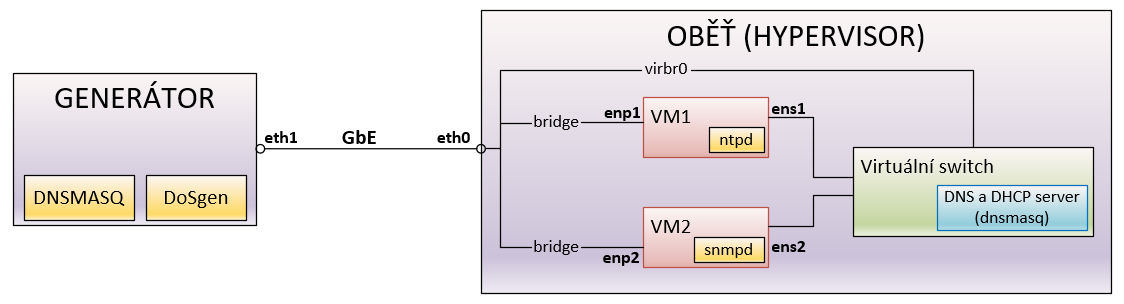
\includegraphics[width=0.9\textwidth]{obrazky/lab_schema.png}
	\caption{Schéma zapojení testovací sítě.}
	\label{fig:vut-lab-schema}
\end{figure}


Stanice vystupující při útoku jako \uv{reflektor} nebo \uv{amplifikátor} a \uv{oběť} jsou plně virtualizované operační systémy skrze hypervizor kernelu (KVM) přistupující ke stejnému síťovému rozhraní \texttt{vnet0}, na něž je připojena i hostitelská stanice. Toto rozhraní je od internetu odděleno prostřednictvím NAT. Pro snazší správu virtualizovaných stanic bylo použito aplikace Virtual Machine Manager ve verzi 1.4.3. V průběhu vývoje a testování jsem využíval nástroje Wireshark pro sledování síťového provozu mezi útočníkem a obětí.

\subsection{Nastavení testovací sítě}
Na hypervizoru bylo použito základní nastavení virtuální sítě. V tomto stavu se virtuální stanice připojují k virtuálnímu switchi v NAT módu. Tento switch je přemostěn přes most \texttt{virbr0} na fyzický síťový adaptér \texttt{eth0}. V této virtuální síti jsou virtuálním stanicím přiřazovány adresy z rozsahu 192.168.122.0/24 programem \texttt{dnsmasq}. Nutno zmínit, že hypervisor má adresu 192.168.122.1. Dále byl pro každou virtuální stanici vytvořen virtuální bridge, který přemosťuje síťová rozhraní \texttt{enp1} a  \texttt{enp2} virtuálních stanic s fyzickým síťovým rozhraním \texttt{eth0} hypervisoru. Takto připojené stanice získávají IP adresy z rozsahu 192.168.2.0/24 a to díky spuštěné službě \texttt{dnsmasq} na serveru DoSgen. Aby bylo možno přistupovat k virtuálním stanicím ze stanice DoSgen, bylo nutné na této stanici do routovací tabulky zapsat statickou cestu do sítě 192.168.122.0/24 přes IP adresu 192.168.2.102.

\subsection{Testování propustnosti sítě}
Tato kapitola se zabývá testováním propustnosti celé sítě a následně zmiňuje výhody a případné nevýhody obou výše zmíněných zapojení.

Na obou fyzických serverech byl spuštěn Apache HTTP server a do jeho kořenového adresáře umístěn binární soubor o velikosti 1 GB. Následně byl z každé stanice tento soubor stažen pomocí programu \texttt{wget}, který zobrazuje rychlost stahování v jednotkách MB/s. Díky této jeho vlastnosti bylo možné změřit propustnost všech spojení v nastavené síti. Data z tohoto testování jsou uvedeny v tabulce \ref{tab:troughput-lab-interfaces}.

\begin{table}[ht]
	\centering
	\caption{Propustnost mezi jednotlivými rozhraními (uvedeno v Mb/s).}
	\label{tab:troughput-lab-interfaces}
	\begin{tabular}{|l|l|l|l|l|}
		\hline
		Rozhraní & eth1 & eth0  & enp1  & ens1  \\ \hline
		eth1     &      & 941   & 525   & 940   \\ \hline
		eth0     & 941  &       & 19200 & 19200 \\ \hline
		enp1     & 525  & 19200 &       & 19200 \\ \hline
		ens1     & 940  & 19200 & 19200 &       \\ \hline
	\end{tabular}
\end{table}

Z těchto dat lze spatřit, že propustnost mezi stanicemi připojenými do virtuálního switche je 2.4 Gb/s a propustnost mezi rozhraními \texttt{eth0} a \texttt{eth1} činí 941 Mb/s. Pokud však generujeme útok ze stanice DoSgen a cílíme jej na virtuální stanici skrze virtuální switch, bude maximální propustnost limitována propustností mezi rozhraními \texttt{eth0} a \texttt{eth1}.
Při využití přemostěného spojení skrze rozhraní \texttt{enp1} a \texttt{enp2} bylo dosaženo maximální propustnosti 525 Mb/s. Jelikož předchozí uvedené zapojení dosáhlo vyšší propustnosti, byly tyto spojení spolu se síťovými rozhraními odstraněny a při testování útoků nebyly využity.

%instalace netdata
%testovani probiha z prikazoveho radku, popsat proc


\subsection{Použitý software} %strucne ke kazdemu co, k cemu, proc jsem zvolil, licence

\newpage
\section{Testování útoku NTP Flood}
Operační systém na kterém je spuštěn NTP sever jsem musel zvolit Fedora 14 jejíž datum vydání bylo 2.\ 11.\ 2010. Bylo nutno zvolit takto starou verzi z důvodu opravy chyby v balíčku \texttt{ntp} v pozdějších vydáních. Nainstalován byl tedy balíček \texttt{ntp-4.2.6p3}. Na tomto stroji musel být správně nakonfigurován firewall tak, abych byl schopen službu NTP kontaktovat z jiné stanice. Následně byl změněn konfigurační soubor pro NTP server způsobem popsaným v kapitole \ref{subsec:ntp_flood}.

Na serveru, který slouží jako oběť tohoto útoku je spuštěn operační systém Fedora 26 Server a nainstalován Apache server ve verzi \texttt{httpd-2.4.29}. Firewall je také patřičně nakonfigurován.

Dalším krokem je vygenerování falešných uživatelů dotazujících se na NTP server. To provedeme spuštěním skriptu a následně si můžeme ověřit pomocí příkazu \texttt{ntpdc}, že záznamů je požadované množství. Pro spuštění těchto příkazů je nutno mít nainstalované balíčky \texttt{net-snmp-utils} a \texttt{python3-scapy}.

\begin{lstlisting}[language=bash]
python3 fake_ntp_hosts.py
ntpdc -n -c monlist 192.168.124.14 | wc -l
\end{lstlisting}

\noindent V tomto okamžiku nic nebrání spuštění útoku a to následovně:
\begin{lstlisting}
./dosgen -i virbr0 -P 4 --ntp -s 192.168.124.129 \
	-d 192.168.124.14
\end{lstlisting}

Nyní je NTP server zahlcován dotazy. Odpověďi na ně zasílá na IP adresu oběti. Výstup aplikace DoSgen lze vidět na obrázku \ref{fig:dosgen_run_ntp-img}

\begin{figure} [ht]
	\centering
	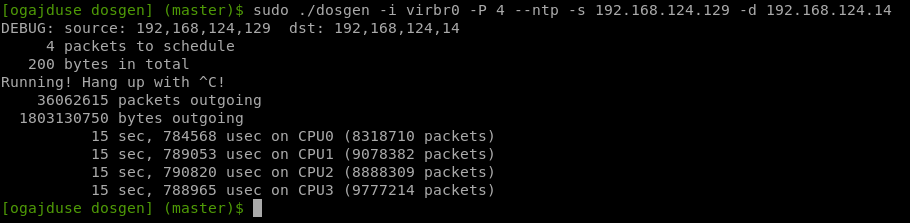
\includegraphics[width=0.9\textwidth]{obrazky/dosgen_terminal_run_ntp.png}
	\caption{Spuštění aplikace DoSgen se zvoleným NTP útokem.}
	\label{fig:dosgen_run_ntp-img}
\end{figure}

Při sledování provozu v programu Wireshark můžeme vidět, že na NTP server je vyslán požadavek \uv{monlist} a NTP server na něj odpovídá, přičemž zamění zdrojovou adresu zamění za cílovou a naopak a paket je tak vyslán na server oběti, která o něj nejeví zájem, tudíž na každý z nich odpovídá ICMP zprávou typu 3 s kódem 9 (Host administratively prohibited). Server je tak zaměstnán odesíláním těchto zpráv a je tedy vyčerpána šířka pásma, dochází k DoS útoku.

\begin{figure} [h]
	\centering
	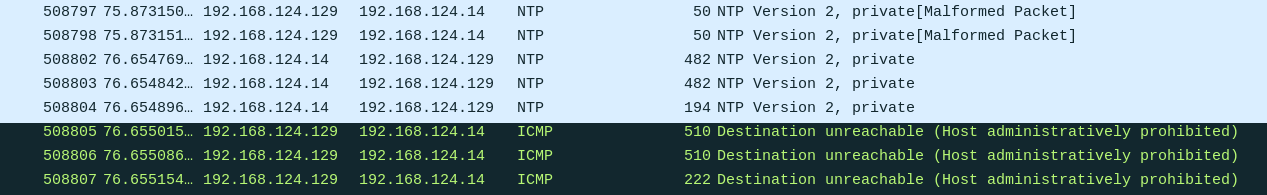
\includegraphics[width=0.9\textwidth]
	{obrazky/mon_getlist_1_wireshark_with_icmp_and_reply.png}
	\caption{Průběh NTP útoku zobrazený v  aplikaci Wireshark.}
	\label{fig:mon_getlist_1_wireshark_with_icmp_and_reply-img}
\end{figure}

Celá tato komunikace je zachycena na obr. \ref{fig:mon_getlist_1_wireshark_with_icmp_and_reply-img}. Pakety s číslem 508797 a 508798 jsou vygenerované nástrojem DoSgen. Následující tři pakety, tedy pakety s číslem 508802-508804 jsou odpovědí NTP serveru. Tato odpověď obsahuje pouze 13 hostů, v případě, že nám server vrátí 600 hostů, odpověď od serveru bude mnohonásobně větší.

Nutno poznamenat, že na serveru oběti musela být uměle modifikována šířka pásma a to na 100 Mbit/s v obou směrech.

\section{Testování útoku SNMP Flood}




%ntpdc -n -c monlist 3.cz.pool.ntp.org

%% Vložení souboru 'text/zaver' se závěrem
% !TeX spellcheck = cs_CZ
\chapter{Závěr}
V této práci se zabývám rozšířením generátoru kybernetických útoků o nové útoky. V úvodu této práce jsou definovány kybernetické útoky obecně, útoky, které následně implementuji, jsou popsány detailněji. Práce detailně popisuje typy kybernetických útoků, jejich různé formy a dělení. Je vysvětlen cíl kybernetických útoků, kdo za nimi stojí a jakým způsobem jsou vykonávany.

V druhé části této se zabývám samotným popisem rozšíření nástroje DoSgen, popisuji jeho strukturu a možnosti použití pro mnou zvolené útoky. Dále se zabývám popisem implementace konkrétních útoků a jejich použitím.

V poslední kapitole se věnuji testování nově implementovaných útoků. Jsou přiloženy snímky obrazovky z průběhu testování.

Ve výsledku se mi podařilo implementovat a řádně otestovat pouze jeden útok, jelikož jsem neodhadl komplexnost této práce.

Dále se plánuji zabývat implementaci zbylých nedokončených útoků, konkrétně SNMP a SSDP. Jedním z dalších mých cílů je restrukturalizace kódu, aktualizace nástroje trafgen implementovaného v DoSgenu a vytvoření manuálové stránky pro DoSgen. V neposlední řadě plánuji vytvořit RPM balíček pro Red Hat Linuxové distribuce.

%% Vložení souboru 'text/literatura' se seznamem literatury
% Pro sazbu seznamu literatury použijte jednu z následujících možností

%%%%%%%%%%%%%%%%%%%%%%%%%%%%%%%%%%%%%%%%%%%%%%%%%%%%%%%%%%%%%%%%%%%%%%%%%
%1) Seznam citací definovaný přímo pomocí prostředí literatura / thebibliography

\begin{literatura}{99}

\bibitem{pirati_internet}
Parlament 2017 - Dlouhodobý program - Internet. \textit{Pirátská strana} [online]. [cit. 2017-11-19]. Dostupné z: https://www.pirati.cz/program/dlouhodoby/internet/

\bibitem{Jirasek2012}
JIRÁSEK, Petr, Luděk NOVÁK a Josef POŽÁR. \textit{Výkladový slovník kybernetické bezpečnosti}. Praha: Policejní akademie ČR v Praze, 2012. ISBN 978-80-7251-378-9.

\bibitem{akamai_q2_2017}
State of the Internet / security Q2 2017 Report. In: ARTEAGA, Jose, Dave LEWIS, Chad SEAMAN, et al. \textit{State of the Internet: Quarterly Security Reports} [online]. 2017, s.~2 [cit. 2017-11-21]. Dostupné z: https://www.akamai.com/uk/en/multimedia/documents/state-of-the-internet/q2-2017-state-of-the-internet-security-report.pdf


\end{literatura}


%%%%%%%%%%%%%%%%%%%%%%%%%%%%%%%%%%%%%%%%%%%%%%%%%%%%%%%%%%%%%%%%%%%%%%%%%
%%2) Seznam citací pomocí BibTeXu
%% Při použití je nutné v TeXnicCenter ve výstupním profilu aktivovat spouštění BibTeXu po překladu.
%% Definice stylu seznamu
%\bibliographystyle{unsrturl}
%% Pro českou sazbu lze použít styl czechiso.bst ze stránek
%% http://www.fit.vutbr.cz/~martinek/latex/czechiso.tar.gz
%%\bibliographystyle{czechiso}
%% Vložení souboru se seznamem citací
%\bibliography{text/literatura}
%
%% Následující příkaz je pouze pro ukázku sazby literatury při použití BibTeXu.
%% Způsobí citaci všech zdrojů v souboru odkazy.bib, i když nejsou citovány v textu.
%\nocite{*}

%% Vložení souboru 'text/zkratky' se seznam použitých symbolů, veličin a zkratek
\begin{seznamzkratek}{Distributed Reflection Denial of Service}

	\novazkratka{zk_dos}
		{DoS}
		{Denial of Service}

	\novazkratka{zk_ddos}
		{DDoS}
		{Distributed Denial of Service}

	\novazkratka{zk_drdos}
		{DRDoS}
		{Distributed Reflection Denial of Service}

	\novazkratka{zk_ddosaas}
		{DDoSaaS}
		{Denial of Service as Service}

	\novazkratka{zk_cnc}
		{C\&C} %mezera ok?
		{Command and Control}

	\novazkratka{zk_irc}
		{IRC}
		{Internet Relay Chat}

	\novazkratka{zk_im}
		{IM}
		{Instant messaging}

	\novazkratka{zk_ntp}
		{NTP}
		{Network Time Protocol}

	\novazkratka{zk_http}
		{HTTP}
		{Hypertext Transfer Protocol}

	\novazkratka{zk_tcp}
		{TCP}
		{Transmission Control Protocol}

	\novazkratka{zk_udp}
		{UDP}
		{User Datagram Protocol}

	\novazkratka{zk_ip}
		{IP}
		{Internet Protocol}

	\novazkratka{zk_icmp}
		{ICMP}
		{Internet Control Message Protocol}

	\novazkratka{zk_smtp}
		{SMTP}
		{Simple Mail Transfer Protocol}
		
	\novazkratka{zk_snmp}
		{SNMP}
		{Simple Network Management Protocol}
	
	\novazkratka{zk_cve}
		{CVE}
		{Common Vulnerabilities and Exposures}
\end{seznamzkratek}


%% Začátek příloh
\prilohy

%% Vysázení seznamu příloh
\seznampriloh

%% Vložení souboru 'text/prilohy' s přílohami
\chapter{Dokumentace nástroje DoSgen}
%makefiles zminit

\section{Instalace}
V této kapitole bude popsána instalace nástroje DoSgen na operačním systému Fedora. Jsou zde zmíněny knihovny, jež je třeba instalovat pro jeho plnou funkčnost. 

\subsection{Instalace závislostí}
\noindent Instalace následujících knihoven je nutností, jelikož jsou přímými závislostmi nástroje trafgen. Výjimkou je knihovna \texttt{libssh}, na které je závislý slovníkový útok.
\begin{lstlisting}[language=bash]
dnf -y install flex bison libnl3-devel libssh-devel
\end{lstlisting}

\noindent Dále je třeba nainstalovat nástroje potřebné ke kompilaci kódu.
\begin{lstlisting}[language=bash]
dnf -y install make pkg-config gcc-c++
\end{lstlisting}

\noindent Chceme-li sestavit dokumentaci k nástroji DoSgen, je nutné mít nainstalován balíček \texttt{rubygem-ronn}, jež zajišťuje konverzi manuálové stránky z jednoduše formátovaného souboru v jazyce Markdown do formátu \texttt{roff}, který je používán pro psaní manuálových stránek.

\begin{lstlisting}[language=bash]
dnf -y install rubygem-ronn
\end{lstlisting}

\noindent Webové rozhraní je závislé na \texttt{nodejs} a \texttt{npm} balíčcích.
\begin{lstlisting}[language=bash]
dnf -y install nodejs npm
\end{lstlisting}



\noindent Instalace následujících balíčků je pouze volitelné, jde o užitečné nástroje, které najdou své místo vedle nástroje DoSgen.
\begin{lstlisting}[language=bash]
dnf -y install tcptrack nmap httping john iftop nload \
ntp net-snmp-utils iputils net-tools
\end{lstlisting}

\subsection{Kompilace}
\noindent Dále je potřeba přeložit zdrojový kód. V rámci této práce byly vyvinuty soubory \texttt{Makefile} v každém podadresáři kořenového adresáře. V kořenovém adresáři se nachází hlavní \texttt{Makefile}, který spouští všechny Makefile obsažené v podadresářích. Tyto soubory obsahují příkazy pro kompilaci a instalaci kódu a zajišťují správné pořadí jejich vykonání.

\begin{lstlisting}[language=bash]
make
\end{lstlisting}

V rámci této práce byl vytvořen také Dockerfile, pomocí kterého lze sestavit kontejner s nainstalovaným nástrojem DoSgen. Výhoda tohoto kontejneru spočívá v tom, že procesy spuštěné v kontejneru jsou oddělené od procesů v hostitelské stanici. Tento kontejner staví na operačním systému Fedora ve verzi 27. Sestavení kontejneru a jeho spuštění lze docílit následovně.
\begin{lstlisting}
docker build -t <NÁZEV_OBRAZU_KONTEJNERU> .
docker run <NÁZEV_OBRAZU_KONTEJNERU>
\end{lstlisting}

\subsection{Webové rozhraní}
Pro spuštění webového rozhraní je nutno nainstalovat Node.js balíčky.
\begin{lstlisting}[language=bash]
cd dosgen-web
make install-npm
# nebo
npm install
\end{lstlisting}

Chceme-li spouštět webovou aplikaci jako démona běžícího na pozadí, je nutno nainstalovat inicializační skript \texttt{dosgen-web.init} do adresáře \texttt{/etc/init.d} a enviromentální soubor do \texttt{/etc/sysconfig}. Používáme-li systém se systemd, pak namísto inicializačního skriptu instalujeme jednotku \texttt{dosgen-web.service} do složky \texttt{/usr/lib/systemd/system}.

Tyto kroky není nutné provádět ručně. Pro tento účel je v Makefile patřičný cíl, který provede instalaci těchto souborů.
\begin{lstlisting}[language=bash]
make install
\end{lstlisting}

V souboru s proměnnými prostředí a souboru \texttt{dosgen.js} je nutno nastavit cestu k nástroji DoSgen a jeho binárnímu souboru. V těchto souborech jsou přítomny komentáře, které uživatele navedou.

\subsection{Dokumentace}
Chceme-li si zobrazit manuálovou stránku pro nástroj DoSgen, je třeba provést překlad.
\begin{lstlisting}[language=bash]
cd man
make
\end{lstlisting}

\subsection{RPM balíček}
Kořenový adresář projektu obsahuje soubor \texttt{dosgen.spec}, jež obsahuje kompletní instrukce pro sestavení RPM balíčku pro Linuxové distribuce založené na balíčkovacím systému RPM. Specfile používá příkaz \texttt{make} ke kompilaci zdrojového kódu i jeho následnou instalaci. Pro sestavení balíčku je nutno vytvořit SRPM balíček a poté spustit proces sestavení samotného RPM balíčku. Pro vytvoření výsledného balíčku je možno použít software \texttt{mock}. 

\begin{lstlisting}[language=bash]
make test-srpm
mock -r fedora-rawhide-x86_64 \
rpmbuild/SRPMS/dosgen-*.src.rpm
\end{lstlisting}

\section{Webové rozhraní}
Webové rozhraní lze spustit jako službu na pozadí,

\begin{lstlisting}[language=bash]
service dosgen-web start
\end{lstlisting}

\noindent nebo lze jej spustit přímo z adresáře \texttt{dosgen-web} spuštěním inicializačního skriptu.

\begin{lstlisting}[language=bash]
./dosgen-web.init start
\end{lstlisting}
%todo přidat obrázek webui
Webové rozhraní je dostupné na adrese:
\begin{lstlisting}
https://<IP adresa stanice>:8888
\end{lstlisting}

Po načtení webového rozhraní je nutno přihlásit se údaji zadanými v souboru \texttt{config.json}. Na hlavní stránce v panelu \texttt{Common Settings} je nutno zadat odchozí síťové rozhraní. Čas útoku a počet procesů jsou volitelné. V nabídce \texttt{Add your attack} si lze vybrat požadovaný útok a následně je uživatel vyzván k zadání parametrů pro tento útok v dalším panelu.

Tlačítka \texttt{Run!} a \texttt{Stop!} slouží ke spuštění a zastavení konkrétního útoku.

%TODO ?? \section{Konfigurační jazyk nástroje Trafgen}





\chapter{Obsah přiloženého CD}
% TODO: vlozit pdf
{\small
%
\dirtree{%.
.1 /\DTcomment{kořenový adresář přiloženého CD}.
.2 configure.
.2 Dockerfile.
.2 dosgen.
.3 argsParse.c.
.3 argsParse.cpp.
.3 argsParse.h.
.3 dosgen.c.
.3 httpFlood.cpp.
.3 httpFlood.h.
.3 libdos.h.
.3 Makefile.
.3 packet.
.3 rudy.cpp.
.3 rudy.h.
.3 slowloris.cpp.
.3 slowloris.h.
.3 slowRead.cpp.
.3 slowRead.h.
.3 sshPass.c.
.3 sshPass.h.
.3 trafgen.
.3 trafgen\_configs.h.
.3 trafgenlib.h.
.3 trafgen\_wrapper.c.
.3 trafgen\_wrapper.h.
.2 dosgen-ansible.
.3 ansible.cfg.
.3 hosts.
.3 ntp.yml.
.3 roles.
.4 ntp.
.4 snmp.
.3 snmp.yml.
.2 dosgen.spec.
.2 dosgen-tools.
.2 dosgen-web.
.3 bin.
.4 www.
.3 cert.pem.
.3 config.json.
.3 dosgen-web.env.
.3 dosgen-web.init.
.3 dosgen-web.service.
.3 key.pem.
.3 Makefile.
.3 package.json.
.3 passport.js.
.3 public.
.4 fonts.
.4 images.
.4 javascripts.
.4 stylesheets.
.3 routes.
.4 auth.js.
.4 dosgen.js.
.3 server.js.
.3 views.
.4 dosgen.ejs.
.4 error.ejs.
.4 login.ejs.
.2 machine-provisioning.
.3 ntpserver.
.4 fedora14.
.5 fedora14.ks.
.5 installation\_command.
.2 Makefile.
.2 man.
.3 dosgen.8.ronn.
.3 Makefile.
.3 README.md.
.2 README.md.
}
}

%% Konec dokumentu
\end{document}
